\documentclass[tikz]{standalone}
\usepackage[utf8x]{inputenc}
\usepackage{tikz}
\usetikzlibrary{patterns}
\begin{document}
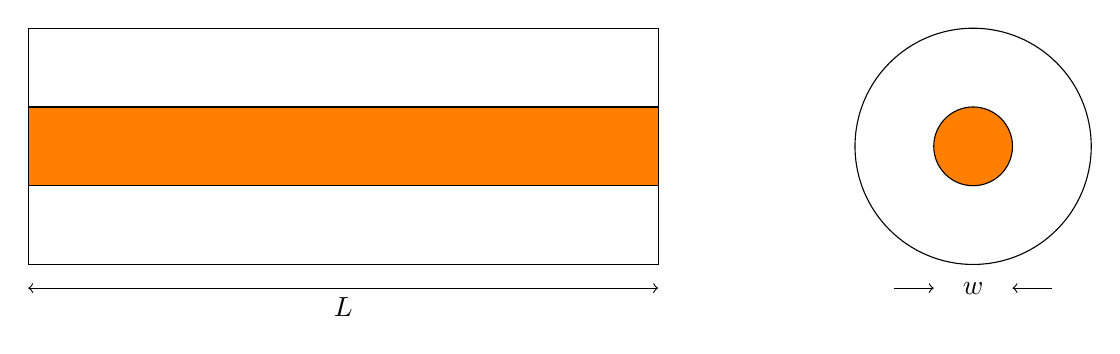
\begin{tikzpicture}[font=\normalsize]
	\draw (0, 0) rectangle (8, 3);
	\draw [fill= red!50!yellow]  (0, 1) rectangle (8, 2);
	\draw [<->] (0, -0.3) -- (8, -0.3) node [below, midway] {$L$};

	\draw (12, 1.5) circle [radius = 1.5];
	\draw [fill= red!50!yellow] (12, 1.5) circle [radius = 0.5];

	\draw (12, -0.3) node {$w$};
	\draw [->] (11, -0.3) -- (11.5, -0.3);
	\draw [<-] (12.5, -0.3) -- (13, -0.3);
\end{tikzpicture}
\end{document}